\chapter{Method}\label{chapter:first_real_chapter}
From a probabilistic point of view, semantic segmentation can be modeled as $p_\theta(x,y)$, where $x$ is a given (rgb-)image, and $y$ is the semantic label. However, in practice there also exist $z$, the physical object of which $x$ is a view. Thus we propose the probabilistic model to be $p_\theta(x,y,z)$. Which can be rewritten as: $p_\theta(x,y,z)$ = $p_\theta(y|x,z) p_\theta(x|z) p_\theta(z)$.
\begin{itemize}
    \item $p_\theta(z)$; The generative process of the object.
    \item $p_\theta(x|z)$; The generative process of the observation of the object.
    \item $p_\theta(y|x,z)$; The generative process of the semantic meaning in the viewport of the observation.
\end{itemize}
Notice that the model $p_\theta(x|z) p_\theta(z)$ is equal to the VAE. We proprose to first learn the generative model $p_\theta(x,z) = p_\theta(x|z) p_\theta(z)$, by learning the approximation of $p_\theta(x|z)$ and $p_\theta(z)$, using a VAE. After which we can use that learnt model to approximate the parameters of $p_\theta(y|x,z)$.

\section{Model}
We start by rewriting the log-likelihood of $p_\theta(x, y, z)$ as shown in Eq.~\ref{eq:label_marginal}. Notice, that the second right hand term, is the log-likelihood of $p_\theta(x)$. Using the Jensen's inequality~~\cite{jensen1906fonctions}, it can be replaced with the $\mathcal{L}_ELBO$. Thus resulting in the $\mathcal{L}_{label-ELBO}$, shown in Eq.~\ref{eq:label_ELBO}

\begin{subequations}
    \begin{align}
        \log p_\theta(x, y) & = \int_z \log p_\theta(y | x, z) dz +  \int_z \log p_\theta(x, z) + \log p_\theta(z) dz             \label{eq:label_marginal} \\
                            & \geq \int_z \log p_\theta(y | x, z) dz + \mathcal{L}_{ELBO}                                                                   \\
                            & = \log p_\theta(y | x) + \mathcal{L}_{ELBO}                                                                                   \\
                            & = \mathbb{E}_{z~q_{\phi}(z | x)}[\log p_\theta(y|x, z)] + \mathcal{L}_{ELBO}                                                  \\
                            & = \mathcal{L}_{label-ELBO} \label{eq:label_ELBO}
    \end{align}
\end{subequations}

Hence, we want to estimate the following three distributions using a neural network.
\begin{itemize}
    \item $q_\phi(z|x)$ (i.e. image encoder)
    \item $p_\theta(x|z)$ (i.e. image decoder)
    \item $p_\theta(y|x, z)$ (i.e. label decoder)
\end{itemize}
We will refer to the image encoder and label decoder together as VAE-Segmentation (VAES). A schematic of the model can be seen in Figure~\ref{fig:schematic-vaes}.

\begin{figure}[h]
    \centering
    \subfloat[A classic VAE and our model during the pre-training phase.\label{fig:schematic-vae}]{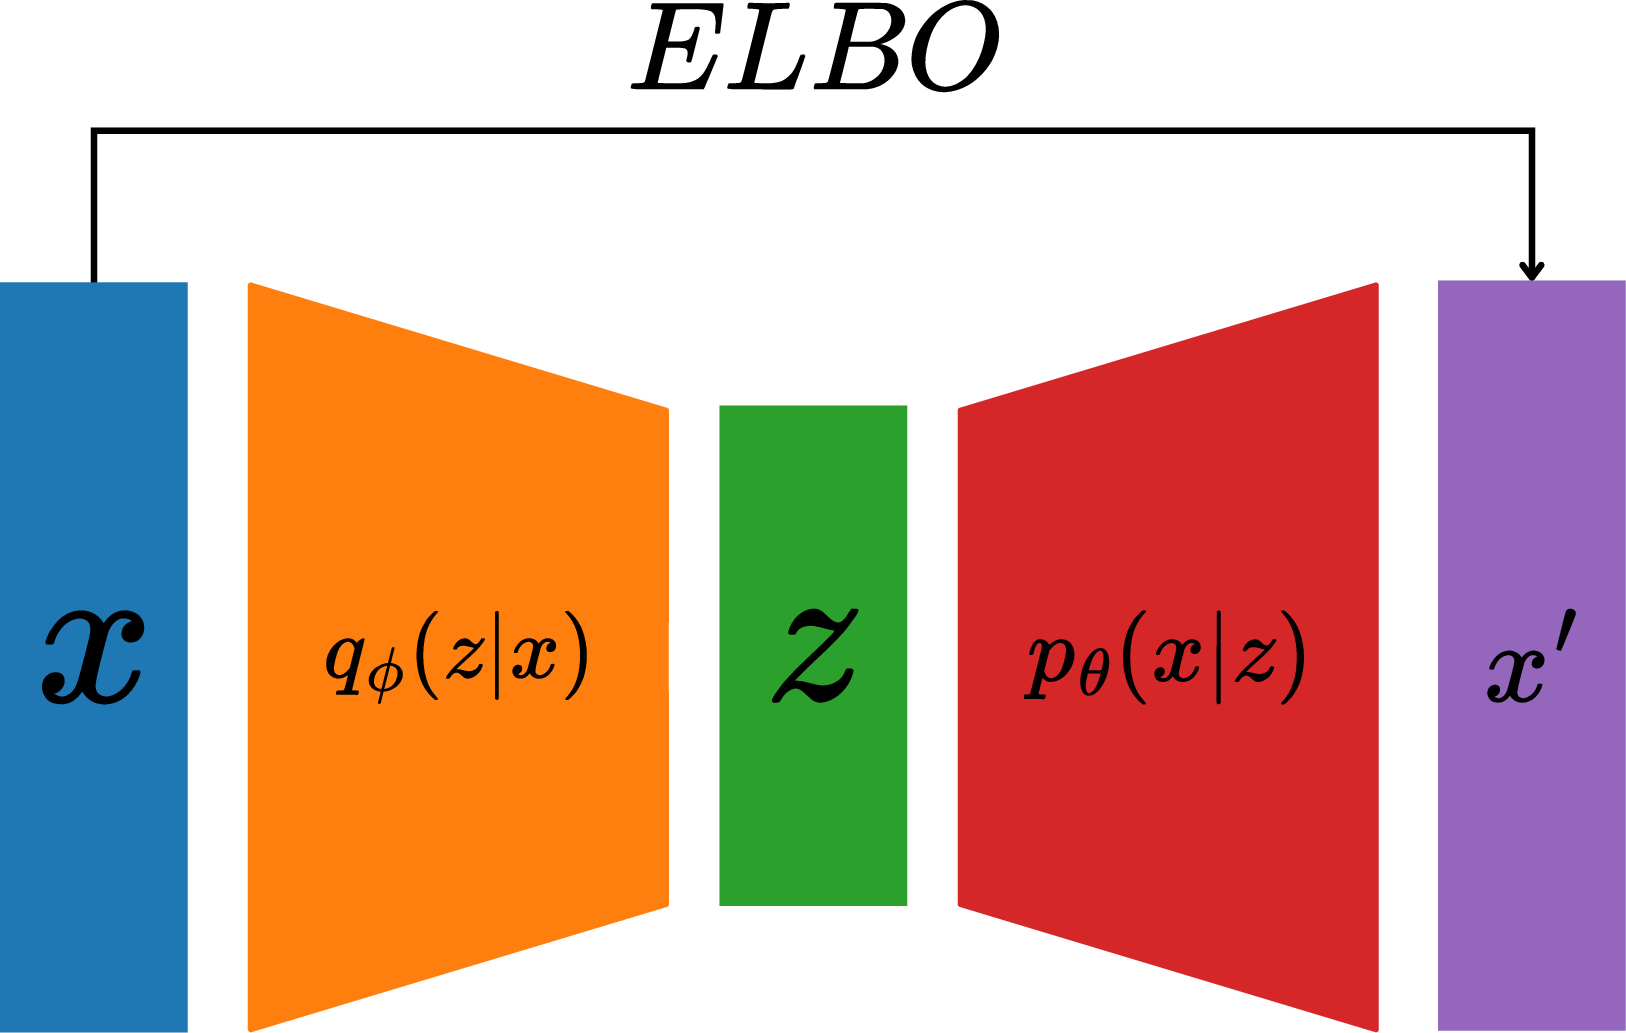
\includegraphics[width=0.45\textwidth]{figures/vae.png}}\hphantom{space}
    \subfloat[The full VAES model. The dotted line shows the skip connections. During inference the image decoder can be disregarded\label{fig:schematic-vaes}]{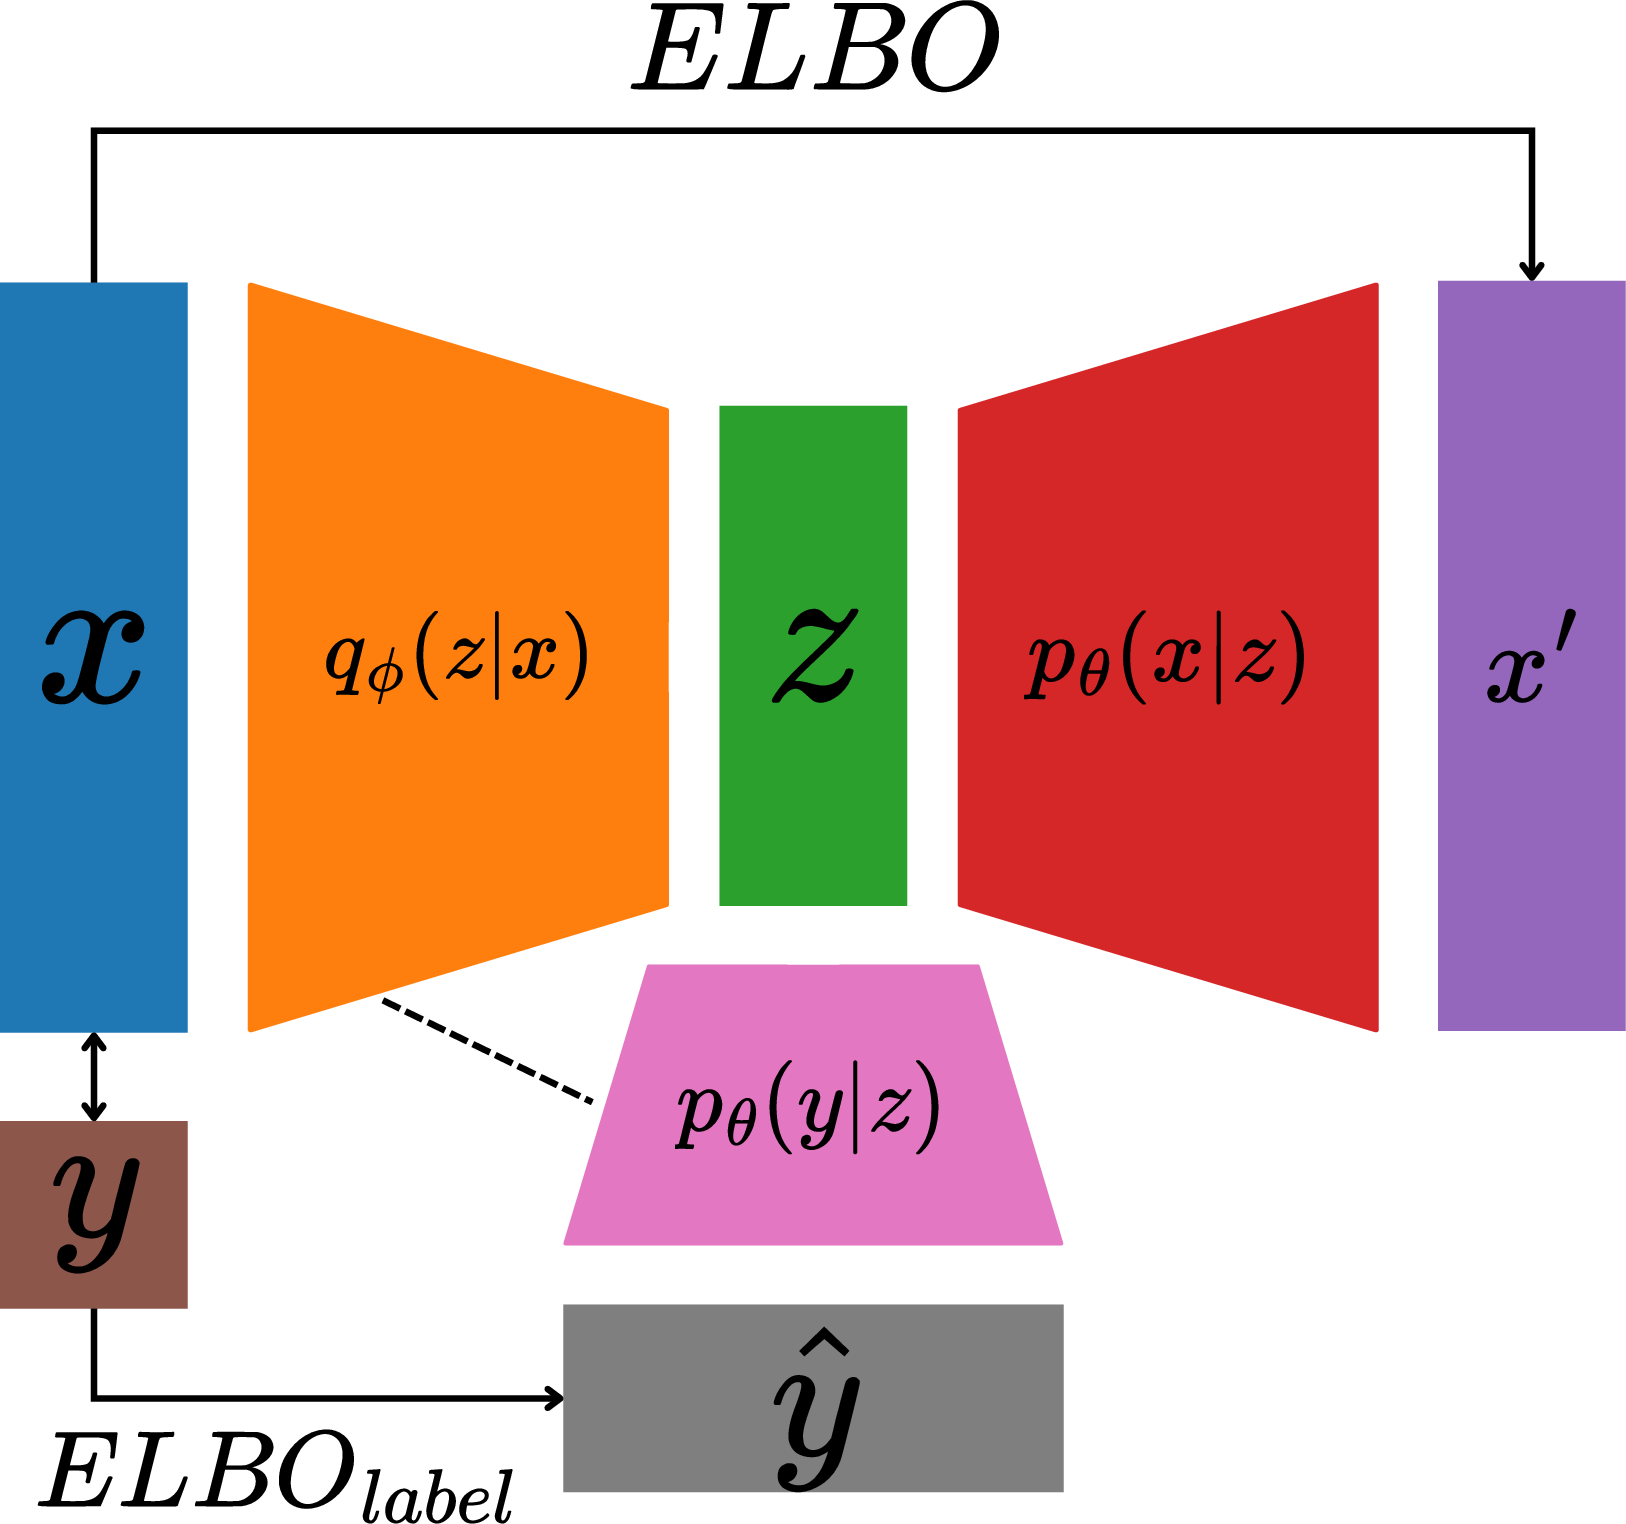
\includegraphics[width=0.45\textwidth]{figures/vaes.png}}
    \caption{A schematic of the proposed VAES.}
\end{figure}

\subsection{Image Encoder}
The image encoder approximates the latent distribution, $p_\theta(z)$. To ensure we can train the encoder using gradient descent, we need to make sure it is fully differentiable. Thus we make use of the reparameterization trick. We use a deterministic mapping $g_\phi(\epsilon, z')$, where $\epsilon$ is an independent random variable and $g_\phi(x)$ is our (deterministic) neural network. Kingma et al.~~\cite{kingma2014autoencodingvariationalbayes} show that using this reparameterization trick a wide range of distributions can be learnt. In our case we use a Gaussian latent space. The reparameterization then becomes $z = \mu + \sigma \epsilon$, where $\mu$ and $\sigma$ are the output of our image encoder network.

\subsection{Image Decoder}
The image decoder approximates the conditional Gaussian distribution $p_\theta(x|z)$. It is used during the pre-training step to prime the image encoder with 'good' initial weights, using the traditional ($\beta$-)VAE training. The hypothesis is, that given that $x$ can be reconstructed from the learnt $q_\phi(z|x)$, the learnt latent space contains useful features to approximate $p_\theta(y|x,z)$. In Eq.~\ref{eq:beta-elbo} $\log p_\theta(x|z)$ can be calculated using Eq.~\ref{eq:log_p_x_z} using a parameterized neural network.

\begin{equation}
    \begin{split}
        \log p_\theta(x|z)      & = \log \mathcal{N}(x; \mu, \sigma^2I) \label{eq:log_p_x_z} \\
        \text{where}~\mu,\sigma & =NN_\theta(z)
    \end{split}
\end{equation}

\subsection{Label Decoder}
The label decoder is similar to the image decoder, except that it approximates a multivariate Bernoulli distribution, instead of a Gaussian. Thus the calculation of $\log p_\theta(y|x,z)$ is different, which is shown in Eq.~\ref{eq:log_p_y_z}. Furthermore, it has `skip connections'. These skip connections allow for information to flow directly from a higher layer in the encoder to the decoder. We make the distinction between 3 types of skip connections.
\begin{enumerate}
    \item Skip. The output of the encoder layer is directly passed to the decoder.
    \item Projection. The output of the encoder layer is first projected using a convolutional layer.
    \item Variational. The output of the encoder layer is first projected using a variational convolutional layer.
\end{enumerate}
When all skip connections are of the type `Skip', our architecture is equal to the UNet architecture.

\begin{subequations}
    \begin{align}
        \log p_\theta(y|x, z) & = \sum_{i=0}^n y_i \log h_i + (1 - y_i)\log(1-h_i) \label{eq:log_p_y_z} \\
        \text{where}~h        & = \text{softmax}(NN_\theta(z))
    \end{align}
\end{subequations}

\section{Training procedure}
The training consist of two stages, the pre-training phase, and the fine-tuning stage. 
\paragraph*{Pre-training phase} During the pre-training phase, the image encoder, $q_\phi(z|x)$, and image decoder, $p_\theta(x|z)$, are trained. This is equal to the classical VAE shown in Figure~\ref{fig:schematic-vae}. The model is optimized to minimise the negative Eq.~\ref{eq:beta-elbo} using stochastic gradient descent with minibatches. Note, that during pre-training no labels are required.

\paragraph*{Fine-tuning phase} During the fine-tuning phase, the learnt image encoder, $q_\phi(z|x)$, is reused. However, the image decoder, $p_\theta(x|z)$, is replaced with a new label decoder, $p_\xi(y|x,z)$. The encoder can either be kept frozen or jointly optimized with the decoder. During fine-tuning the negative of Eq.~\ref{eq:label_ELBO} is minimised.

In the case that the image encoder is kept frozen, the dataset can be encoded once into the latent space. This latent space can then be sampled, reducing the computational and memory required during training.

\section{Evaluation}
\subsection{Inference}
Due to the variational architecture of the model, the inference can be done in two ways. One way is deterministic, by taking the mode of each latent vector. The other is variational, by sampling each latent vector. During training sampling the latent space is useful to improve the stability of training. However, during evaluation it is prefered for the model to be deterministic. Hence during evaluation the mode of the latent space is used.

\subsection{Metrics}
The most well-known and widely-used metrics within classification are precision (Eq.~\ref{eq:precision}), recall (Eq.~\ref{eq:recall}), and F1-score (Eq.~\ref{eq:f1})~\cite{rijsbergen1979information}. The latter is a combination of precision and recall. Within the field of image segmentation is also sometimes referred to as the Recognition Quality (RQ). In this, TP, FP, and FN refer to the True Positive, False Positive, and False Negative predictions per pixel. As our model always gives a prediction for each pixel, an FP in one class will always coincide with an FN in another class. Another common metric is the Jaccard Index (Eq.~\ref{eq:jaccard}), which is monotonically similar to the F1-score, but weigths incorrect predictions more. As they are similar we will only report the Jaccard Index.

\begin{subequations}
    \begin{align}
        \text{Precision}     & = \frac{TP}{TP + FP} \label{eq:precision}                                               \\
        \text{Recall}        & = \frac{TP}{TP + FN} \label{eq:recall}                                                  \\
        F1 = \text{RQ}       & = 2 \cdot \frac{\text{Precision} \cdot \text{Recall}}{\text{Precision} + \text{Recall}} \\ 
                             & = \frac{TP}{\frac{1}{2} (FN + FP) + TP} \label{eq:f1}                                   \\
        \text{Jaccard Index} & = \frac{TP}{FN + FP + TP} \label{eq:jaccard}
    \end{align}
\end{subequations}
